\documentclass[12pt, a4paper]{article}

\usepackage{graphicx}
\usepackage{float}
\usepackage{hyperref}

\hypersetup{
	colorlinks=true,
	linkcolor=black
}


\begin{document}
	\pagenumbering{gobble}
	\begin{titlepage}
		\makebox[\textwidth]{\large  Department of Electrical and Electronic Engineering}
		\vspace*{1.5cm}
		\makebox[\textwidth]{\large University of Johannesburg}
		\makebox[\textwidth]{\textbf{EEP3B21 2018}}
		\vspace*{1.5cm}
		\makebox[\textwidth]{\textit{Lecturer: Dr. AR Ndjiongue}}
		\makebox[\textwidth][l]{\large ELECTRONICS}
		\vspace*{1.5cm}
		\makebox[\textwidth][r]{\large Group Project}
		\vspace*{0.5cm}
		\makebox[\textwidth]{\LARGE Group Project 2 Report}
		\vspace*{0.1cm}
		\makebox[\textwidth]{\large Ruan de Bruyn - 216054484}
		\vspace*{0.1cm}
		\makebox[\textwidth]{\large Quintin Kruger - 216054484}
		\vspace*{0.1cm}
		\makebox[\textwidth]{\large Wesley Richardson - 216054484}
		\vspace*{0.3cm}
		\makebox[\textwidth]{\today}
		\vfill
		\noindent I hereby declare that, except where specifically indicated, the work submitted herein is my own original work\\
		Signed: \hspace*{5cm} Date:
	\end{titlepage}

	\pagenumbering{roman}
	\tableofcontents
	\newpage
	\pagenumbering{arabic}

\section{Theoretical Background}

	\subsection{Modulator}
	\subsection{Demodulator Circuit}
		A demodulator circuit is one of the applications of a diode as a detector for amplitude modulated (AM) radio signals. An AM signal consists of a radio-frequency carrier wave whose amplitude varies with different audio frequencies.

		The detector circuit circuit is essentially a half-wave rectifier circuit with an RC filter placed on the output as can be seen from the circuit of the modulator circuit for this practical in Figure \ref{demodulator_circuit}.

		The RC time constant of the filter should fall between 2 values
		\begin{equation}
			\frac{1}{\omega_c} \le RC \le \frac{\sqrt{1-\mu^2}}{\omega_m\mu}
		\end{equation}

		where $\omega_c$ is the frequency of the carrier, $\omega_m$ is the angular frequency of the information and $\mu$ is the modulation index

		This result comes from practical experience in the field of electronic engineering rather than from a mathematical principles.

		If the $RC$ time constant is too small, there would be ripples of the carrier frequency on the output (this is to be avoided as we require the information sent rather than the distortion thereof with the carrier signal).

		If the $RC$ time constant is too big, it will significantly attenuate high frequencies 


		\begin{figure}[H]
			\centering
			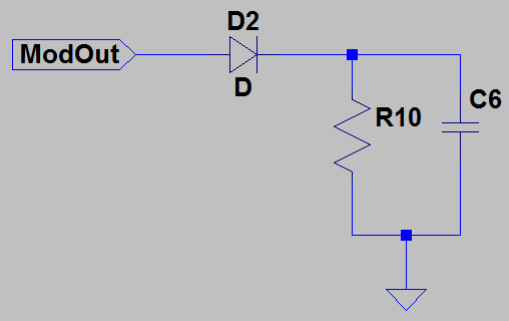
\includegraphics[width=0.7\textwidth]{images/Demodulator_circuit.png}
			\caption{The demodulator circuit used for this experiment}
			\label{demodulator_circuit}
		\end{figure}

	\subsection{}

\section{Experimental Method} % (fold)
\label{sec:experimental_method}
	
% section experimental_method (end)

\section{Results} % (fold)
\label{sec:results}
	\begin{figure}[H]
		\centering
		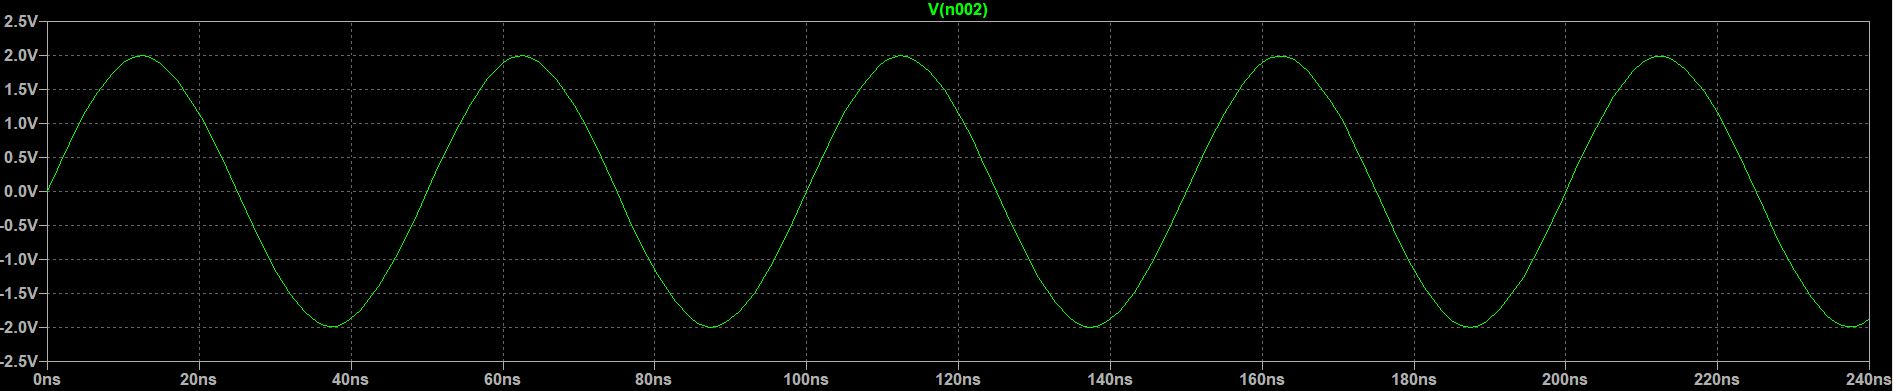
\includegraphics[width=.8\textwidth]{images/carrier.JPG}
		\caption{20 MHz Carrier signal}
		\label{fig:carrier}
	\end{figure}

	\begin{figure}[H]
		\centering
		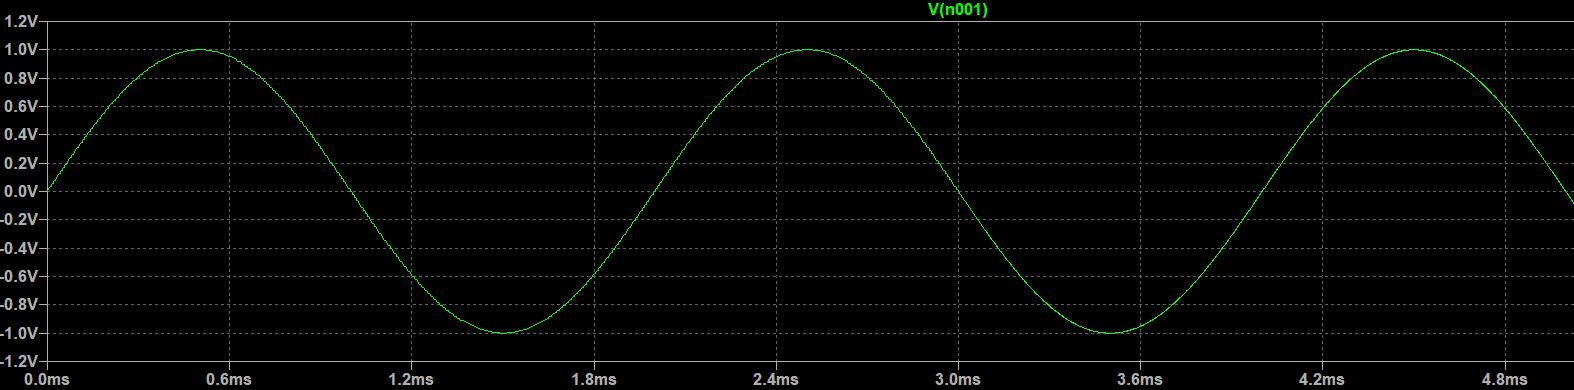
\includegraphics[width=.8\textwidth]{images/modulating.JPG}
		\caption{500 Hz input signal}
		\label{fig:modulating}
	\end{figure}

	\begin{figure}[H]
		\centering
		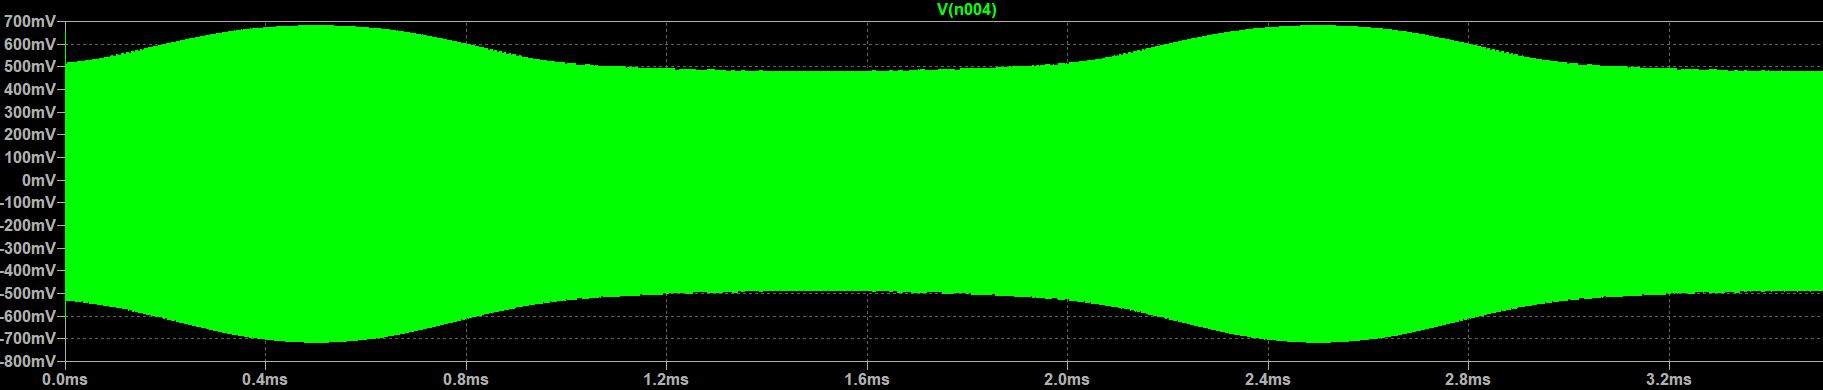
\includegraphics[width=.8\textwidth]{images/output_modulated.JPG}
		\caption{Modulator output}
		\label{fig:output_modulated}
	\end{figure}

	\begin{figure}[H]
		\centering
		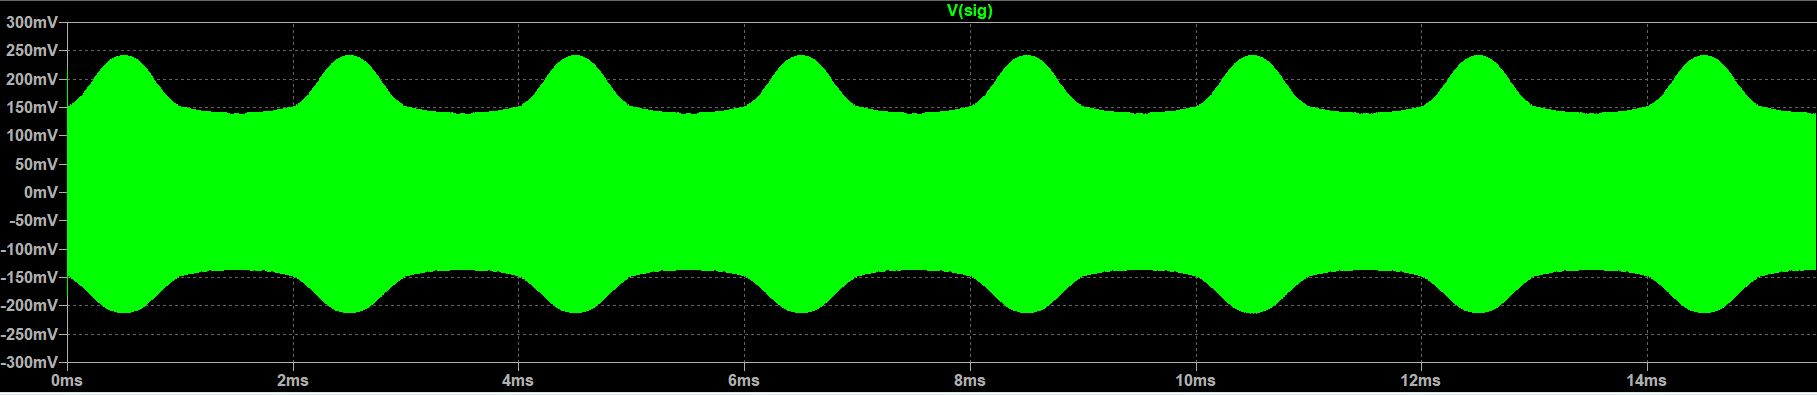
\includegraphics[width=.8\textwidth]{images/output_demodulated.JPG}
		\caption{Demodulated output}
		\label{fig:output_demodulated}
	\end{figure}
% section results (end)

\section{Discussion} % (fold)
\label{sec:discussion}
	In this practical, we have chosen the carrier wave with a frequency of 20 MHz, and an amplitude of $5V$. In order to simulate audio input, we simply chose a signal generator which generates a 500 Hz sine wave at an amplitude of $1V$. These two signals can be seen in Figure \ref{fig:carrier} and Figure \ref{fig:modulating}. What we expect at the modulated output of the circuit, theoretically, is to have a 20 MHz signal that has the envelope of the 500 Hz sine wave input. From Figure \ref{fig:output_modulated} we can see that this is indeed the case.

	The signal looks ``solid'' due to the large difference between the frequencies of the carrier and modulating waves. It is instructive to note that, due to the constraints of the practical, we had to choose a carrier signal that would require the capacitor $C_2$ in the circuit to have a value of $3pF \le C_2 \le 40pF$. Now, since the modulating signal is 500 Hz, we expect the envelope of the carrier signal to have a period once every 2$ms$. By inspecting the voltage values of Figure \ref{fig:output_modulated}, we see that the modulated signal at 0$ms$ is approximately $514mV$. The value of the modulated signal at $2ms$ is also $514mV$. Therefore we can conclude that the envelope of the carrier signal is indeed correct.

	In Figure \ref{fig:output_demodulated} shows the demodulated output of the circuit. By visual inspection, it can still be seen that the signal has an envelope of 500 Hz, as it is periodic, and repeats every $2ms$. From the envelope, however, it appears that the bottom half of the 500 Hz modulating signal is somewhat distorted.

	There is quite a difference in the amplitudes of the modulated and demodulated signals. We would expect, mathematically, that the two signals should have a maximum amplitude of $5V$, as the carrier and modulating signals peak at $5V$ and $1V$ respectively. However, the modulated output signal has a maximum output of around $700mV$, while the demodulated output signal has a maximum signal of approximately $250mV$. One reason for this reduction in voltage is due the modulating and demodulating process. The modulation process has an LC circuit, whose impedance acts to attenuate the voltage of the signal. A voltage drop across the diodes in the circuit also serve to reduce the maximum amplitude of the output voltage. It is clear that this signal will have to be at some stage during the encoding process, so that higher level signals can be obtained.
% section discussion (end)

\section{Conclusion} % (fold)
\label{sec:conclusion}
	
% section conclusion (end)

\begin{thebibliography}{500}

	\bibitem{lamport94}
	  Donald A. Neamen,
	  \textit{Microelectronics: Circuit Analysis and Design}

	\bibitem{Detector}
	Phil Frost
	\textit{RC time constant and diode detector}
	\texttt{https://electronics.stackexchange.com/questions/100518/rc-time-constant-and-diode-detector}

\end{thebibliography}

\end{document}